% move all configuration stuff into includes file so we can focus on the content
\documentclass[aspectratio=169,hyperref={pdfpagelabels=false,colorlinks=true,linkcolor=white,urlcolor=blue},t]{beamer}

%%%%%%%%%%%%%%%%%%%%%%%%%%%%%%%%%%%%%%%%%%%%%%%%%%%%%%%%%%%%%%%%%%%%%%%%%%%%%%%%%%
%%%%%%%%%%%%%%%%%%%%%%%%%%%%%%%%%%%%%%%%%%%%%%%%%%%%%%%%%%%%%%%%%%%%%%%%%%%%%%%%%%
% packages
\usepackage{pict2e}
\usepackage{epic}
\usepackage{amsmath,amsfonts,amssymb}
\usepackage{units}
\usepackage{fancybox}
\usepackage[absolute,overlay]{textpos} 
\usepackage{media9} % avi2flv: "C:\Program Files\ffmpeg\bin\ffmpeg.exe" -i TuneFreqFilterbank.avi -b 600k -s 441x324 -r 15 -acodec copy TuneFreqFilterbank.flv
\usepackage{animate}
\usepackage{gensymb}
\usepackage{multirow}
\usepackage{silence}
\usepackage[backend=bibtex,style=ieee]{biblatex}
\AtEveryCitekey{\iffootnote{\tiny}{}}
\addbibresource{references}

%%%%%%%%%%%%%%%%%%%%%%%%%%%%%%%%%%%%%%%%%%%%%%%%%%%%%%%%%%%%%%%%%%%%%%%%%%%%%%%%%%
%%%%%%%%%%%%%%%%%%%%%%%%%%%%%%%%%%%%%%%%%%%%%%%%%%%%%%%%%%%%%%%%%%%%%%%%%%%%%%%%%%
% relative paths
\graphicspath{{graph/}}


%%%%%%%%%%%%%%%%%%%%%%%%%%%%%%%%%%%%%%%%%%%%%%%%%%%%%%%%%%%%%%%%%%%%%%%%%%%%%%%%%%
%%%%%%%%%%%%%%%%%%%%%%%%%%%%%%%%%%%%%%%%%%%%%%%%%%%%%%%%%%%%%%%%%%%%%%%%%%%%%%%%%%
% units
\setlength{\unitlength}{1mm}

%%%%%%%%%%%%%%%%%%%%%%%%%%%%%%%%%%%%%%%%%%%%%%%%%%%%%%%%%%%%%%%%%%%%%%%%%%%%%%%%%%
%%%%%%%%%%%%%%%%%%%%%%%%%%%%%%%%%%%%%%%%%%%%%%%%%%%%%%%%%%%%%%%%%%%%%%%%%%%%%%%%%%
% theme & layout
\usetheme{Frankfurt}
\beamertemplatenavigationsymbolsempty
%\setbeamertemplate{frametitle}[smoothbars theme]
\setbeamertemplate{frametitle}
{
    \begin{beamercolorbox}[ht=1.8em,wd=\paperwidth]{frametitle}
        \vspace{-.1em}%
        \hspace{.2em}{\strut\insertframetitle\strut}
        
        \hspace{.2em}\small\strut\insertframesubtitle\strut
        %\hfill
        %
\includegraphics[height=.8cm,keepaspectratio]{CenterMusicTechnology-solid-2lines-white-CoAtag}
        
    \end{beamercolorbox}
    \begin{textblock*}{100mm}(11.6cm,.7cm)
        \includegraphics[height=.8cm,keepaspectratio]{logo_GTCMT_black}
    \end{textblock*}
}

% set this to ensure bulletpoints without subsections
\usepackage{remreset}
\makeatletter
\@removefromreset{subsection}{section}
\makeatother
\setcounter{subsection}{1}

%---------------------------------------------------------------------------------
% appearance
\setbeamercolor{structure}{fg=gtgold}
\setbeamercovered{transparent} %invisible
\setbeamercolor{bibliography entry author}{fg=black}
\setbeamercolor*{bibliography entry title}{fg=black}
\setbeamercolor*{bibliography entry note}{fg=black}

%\usepackage{pgfpages}
%\setbeameroption{show notes}
%\setbeameroption{show notes on second screen=right}
%---------------------------------------------------------------------------------
% fontsize
\let\Tiny=\tiny

%%%%%%%%%%%%%%%%%%%%%%%%%%%%%%%%%%%%%%%%%%%%%%%%%%%%%%%%%%%%%%%%%%%%%%%%%%%%%%%%%%
%%%%%%%%%%%%%%%%%%%%%%%%%%%%%%%%%%%%%%%%%%%%%%%%%%%%%%%%%%%%%%%%%%%%%%%%%%%%%%%%%%
% warnings
\pdfsuppresswarningpagegroup=1
\WarningFilter{biblatex}{Patching footnotes failed}
\WarningFilter{latexfont}{Font shape}
\WarningFilter{latexfont}{Some font shapes}
\WarningFilter{gensymb}{Not defining}


%%%%%%%%%%%%%%%%%%%%%%%%%%%%%%%%%%%%%%%%%%%%%%%%%%%%%%%%%%%%%%%%%%%%%%%%%%%%%%%%%%
%%%%%%%%%%%%%%%%%%%%%%%%%%%%%%%%%%%%%%%%%%%%%%%%%%%%%%%%%%%%%%%%%%%%%%%%%%%%%%%%%%
% title information
\title[]{Introduction to Audio Content Analysis}   
\author[alexander lerch]{alexander lerch} 
%\institute{~}
%\date[Alexander Lerch]{}
\titlegraphic{\vspace{-16mm}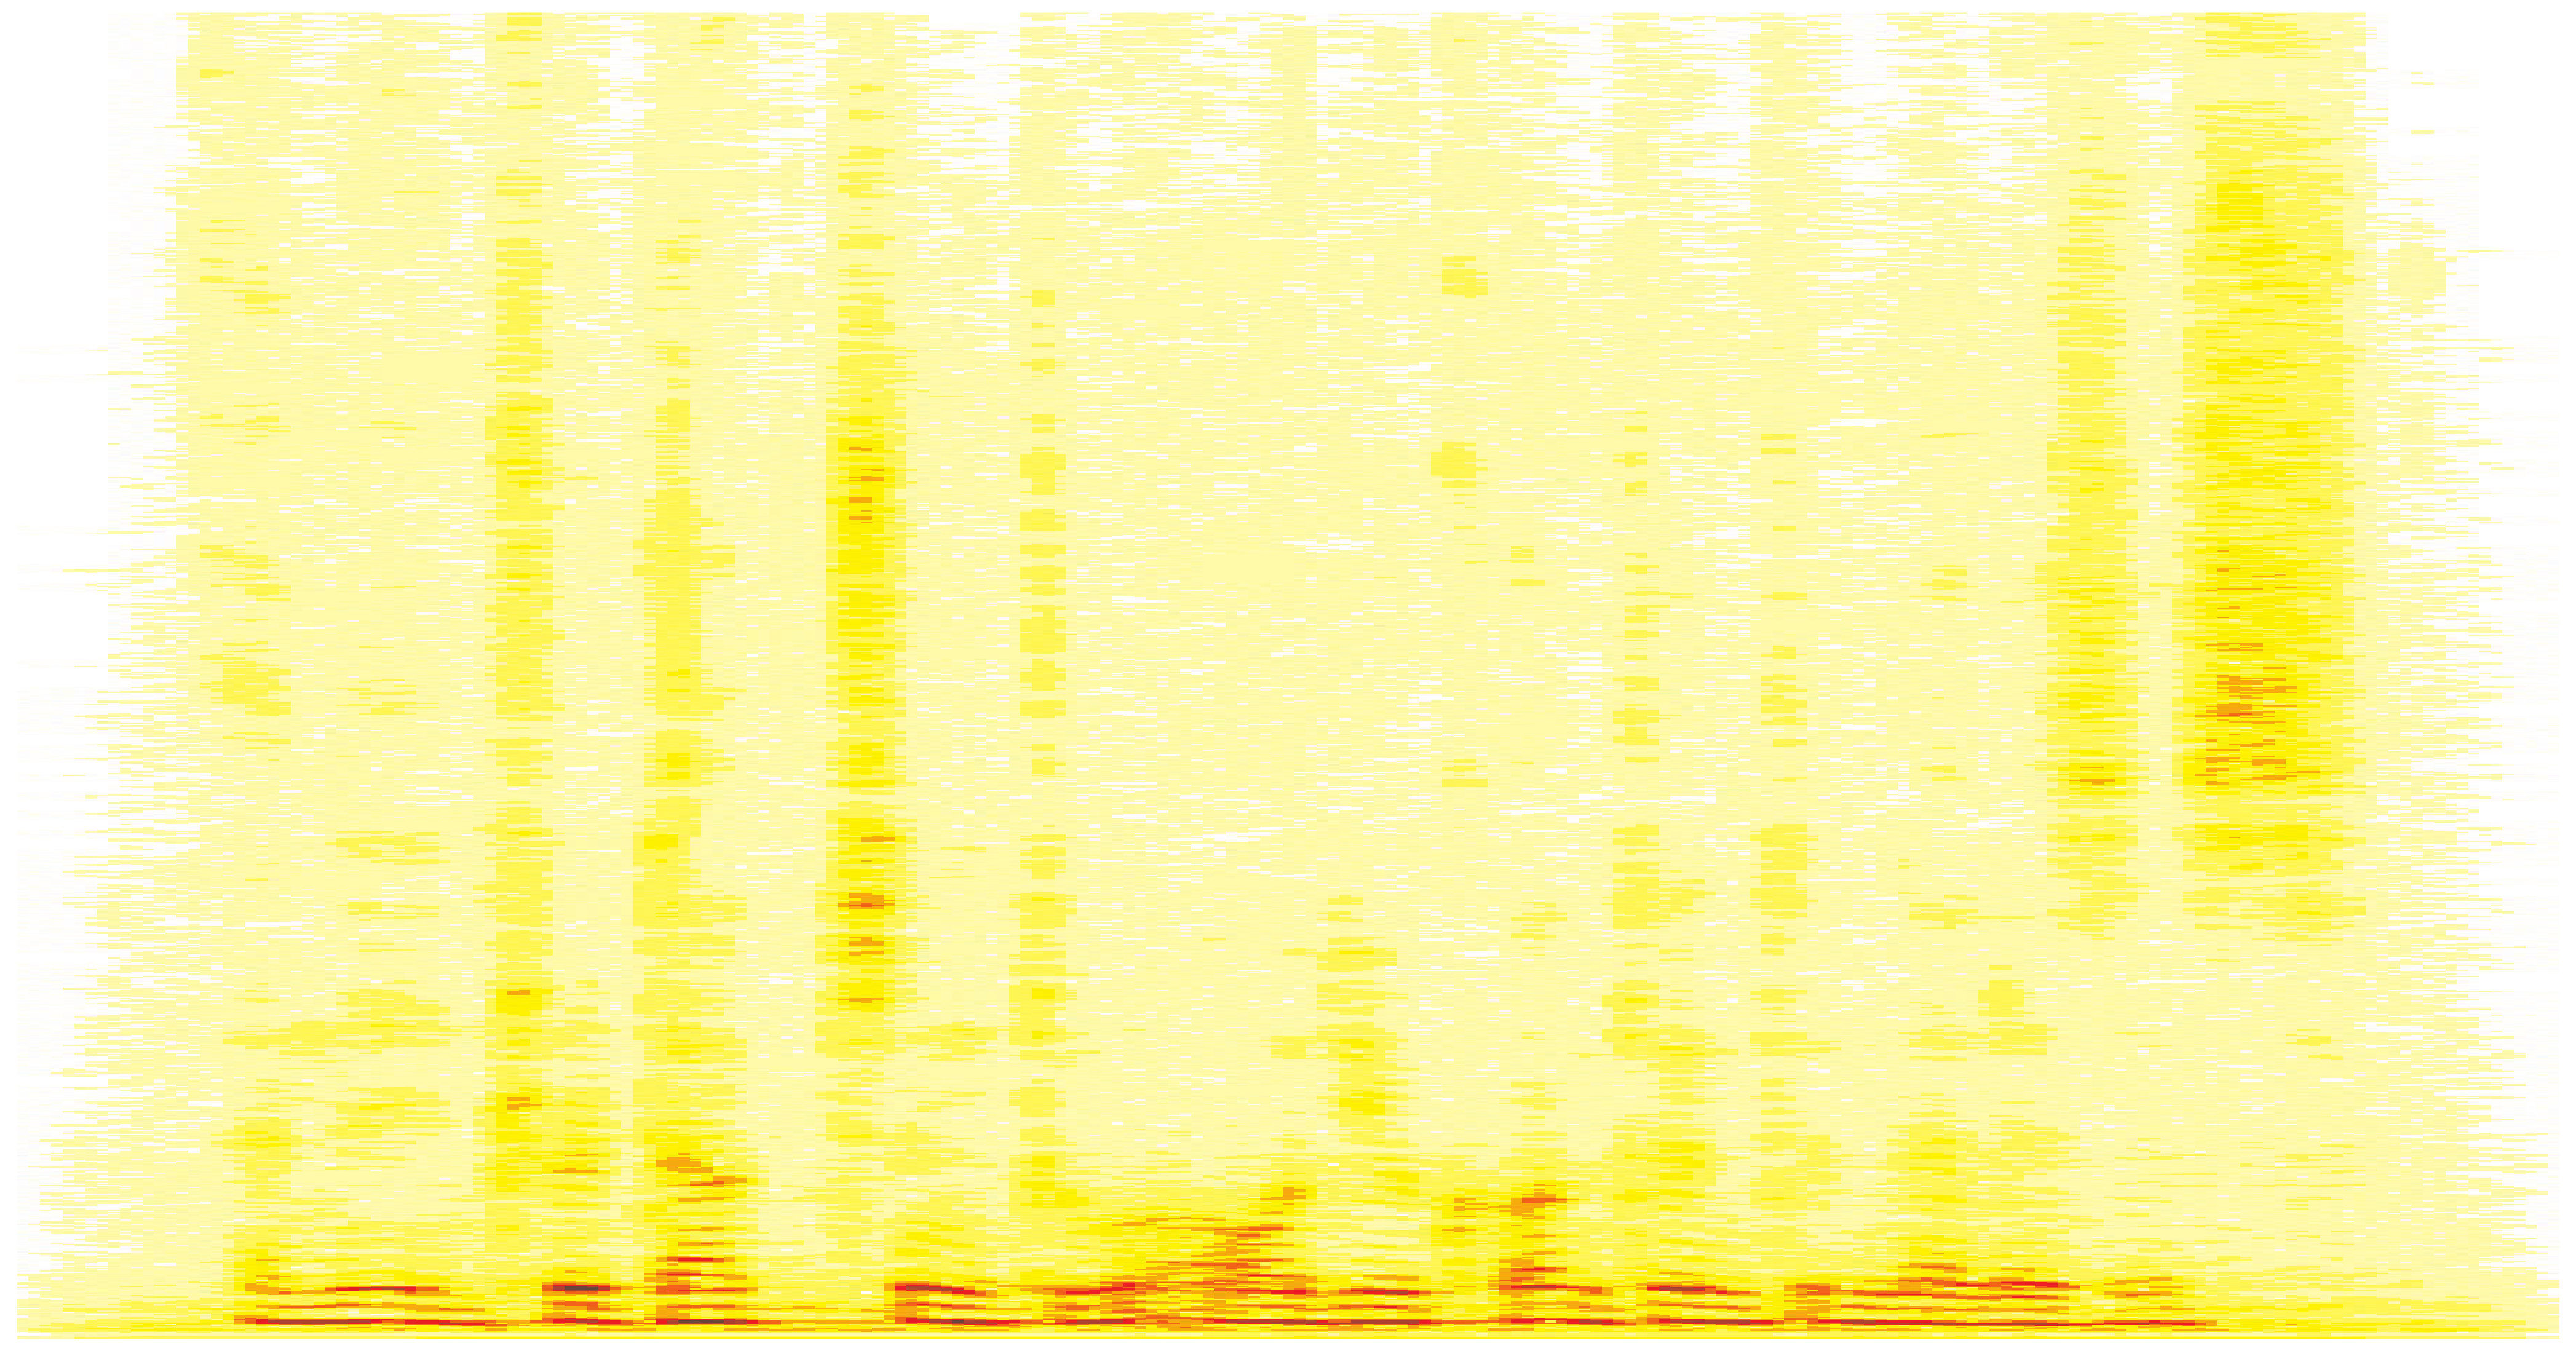
\includegraphics[width=\textwidth,height=3cm]{title}}

%%%%%%%%%%%%%%%%%%%%%%%%%%%%%%%%%%%%%%%%%%%%%%%%%%%%%%%%%%%%%%%%%%%%%%%%%%%%%%%%%%
%%%%%%%%%%%%%%%%%%%%%%%%%%%%%%%%%%%%%%%%%%%%%%%%%%%%%%%%%%%%%%%%%%%%%%%%%%%%%%%%%%
% colors
\definecolor{gtgold}{HTML}{E0AA0F} %{rgb}{0.88,0.66,1,0.06} [234, 170, 0]/256

%%%%%%%%%%%%%%%%%%%%%%%%%%%%%%%%%%%%%%%%%%%%%%%%%%%%%%%%%%%%%%%%%%%%%%%%%%%%%%%%%%
%%%%%%%%%%%%%%%%%%%%%%%%%%%%%%%%%%%%%%%%%%%%%%%%%%%%%%%%%%%%%%%%%%%%%%%%%%%%%%%%%%
% math
\DeclareMathOperator*{\argmax}{argmax}
\DeclareMathOperator*{\argmin}{argmin}
\DeclareMathOperator*{\atan}{atan}
\DeclareMathOperator*{\arcsinh}{arcsinh}
\DeclareMathOperator*{\sign}{sign}
\DeclareMathOperator*{\tcdf}{tcdf}
\DeclareMathOperator*{\si}{sinc}
\DeclareMathOperator*{\princarg}{princarg}
\DeclareMathOperator*{\arccosh}{arccosh}
\DeclareMathOperator*{\hwr}{HWR}
\DeclareMathOperator*{\flip}{flip}
\DeclareMathOperator*{\sinc}{sinc}
\DeclareMathOperator*{\floor}{floor}
\newcommand{\e}{{e}}
\newcommand{\jom}{\mathrm{j}\omega}
\newcommand{\jOm}{\mathrm{j}\Omega}
\newcommand   {\mat}[1]    		{\boldsymbol{\uppercase{#1}}}		%bold
\renewcommand {\vec}[1]    		{\boldsymbol{\lowercase{#1}}}		%bold

%%%%%%%%%%%%%%%%%%%%%%%%%%%%%%%%%%%%%%%%%%%%%%%%%%%%%%%%%%%%%%%%%%%%%%%%%%%%%%%%%%
%%%%%%%%%%%%%%%%%%%%%%%%%%%%%%%%%%%%%%%%%%%%%%%%%%%%%%%%%%%%%%%%%%%%%%%%%%%%%%%%%%
% media9
\newcommand{\includeaudio}[1]{{\includemedia[
                        addresource=audio/#1.mp3,
                        width=5mm,
                        height=5mm,
                        activate=onclick,
                        flashvars={
                            source=audio/#1.mp3  
                            &autoPlay=true
                        }]
                        {
\includegraphics[width=5mm, height=5mm]{SpeakerIcon}}
                        {APlayer.swf}}}
\newcommand{\audioautoplay}[1]{{\begin{center}\includemedia[
                            addresource=audio/#1.mp3,
                            width=.1\linewidth,
                            height=.01\linewidth,
                            activate=pageopen,
                            flashvars={
                                source=audio/#1.mp3  
                                &autoPlay=true
                            }]
                            {}
                            {APlayer.swf}\end{center}}}

\newcommand{\includevideo}[1]{{\begin{center}\includemedia[
                        addresource=video/#1.mp4,
                        width=0.8\linewidth,
                        height=0.4\linewidth,
                        activate=onclick,
                        flashvars={
                            source=video/#1.mp4  
                            &autoPlay=true
                        }]
                        {}
                        {VPlayer.swf}\end{center}}}
\newcommand{\videowithmatlab}[1]{{\begin{center}\includemedia[
                        addresource=video/animate#1.mp4,
                        width=0.8\linewidth,
                        height=0.4\linewidth,
                        activate=onclick,
                        flashvars={
                            source=video/animate#1.mp4  
                            &autoPlay=true
                        }]
                        {}
                        {VPlayer.swf}\end{center}\addreference{matlab source: matlab/animate#1.m}}}
                        

%%%%%%%%%%%%%%%%%%%%%%%%%%%%%%%%%%%%%%%%%%%%%%%%%%%%%%%%%%%%%%%%%%%%%%%%%%%%%%%%%%
%%%%%%%%%%%%%%%%%%%%%%%%%%%%%%%%%%%%%%%%%%%%%%%%%%%%%%%%%%%%%%%%%%%%%%%%%%%%%%%%%%
% other commands
\newcommand{\question}[1]{%\vspace{-4mm}
                          \setbeamercovered{invisible}
                          \begin{columns}[T]
                            \column{.8\textwidth}
                                \textbf{#1}
                            \column{.2\textwidth}
                                \vspace{-8mm}
                                \begin{flushright}
                                     
\includegraphics[scale=.5]{question_mark}
                                \end{flushright}
                                \vspace{6mm}
                          \end{columns}\pause\vspace{-12mm}}

\newcommand{\toremember}[1]{%\vspace{-4mm}
                          \begin{columns}[T]
                            \column{.8\textwidth}
                                \textbf{#1}
                            \column{.2\textwidth}
                                \vspace{-4mm}
                                \begin{flushright}
                                     
\includegraphics[scale=.5]{exclamation_mark}
                                \end{flushright}
                                \vspace{6mm}
                          \end{columns}\vspace{-6mm}}

\newcommand{\matlabexercise}[1]{%\vspace{-4mm}
                          \setbeamercovered{invisible}
                          \begin{columns}[T]
                            \column{.8\textwidth}
                                \textbf{matlab exercise}: #1
                            \column{.2\textwidth}
                                \begin{flushright}
                                     
\includegraphics[scale=.5]{logo_matlab}
                                \end{flushright}
                                %\vspace{6mm}
                          \end{columns}}

\newcommand{\addreference}[1]{  
                  
                    \begin{textblock*}{\baselineskip }(1.12\textwidth,.3\textheight) %(1.15\textwidth,.4\textheight)
                        \rotatebox{90}{\tiny {#1}}
                    \end{textblock*}}
                    
\newcommand{\figwithmatlab}[1]{
                    \begin{figure}
                        \centering
                        \includegraphics{#1}
                        %\label{fig:#1}
                    \end{figure}
                    
                    \addreference{matlab source: \href{https://github.com/alexanderlerch/ACA-Slides/blob/master/matlab/display#1.m}{matlab/display#1.m}}}
\newcommand{\figwithref}[2]{
                    \begin{figure}
                        \centering
                        \includegraphics{#1}
                        \label{fig:#1}
                    \end{figure}
                    
                    \addreference{#2}}  
                                    
\newcommand{\inserticon}[1]{

                    \begin{textblock*}{100mm}(14.5cm,7.5cm)
                        \includegraphics[height=.8cm,keepaspectratio]{#1}
                    \end{textblock*}}            

%%%%%%%%%%%%%%%%%%%%%%%%%%%%%%%%%%%%%%%%%%%%%%%%%%%%%%%%%%%%%%%%%%%%%%%%%%%%%%%%%%
%%%%%%%%%%%%%%%%%%%%%%%%%%%%%%%%%%%%%%%%%%%%%%%%%%%%%%%%%%%%%%%%%%%%%%%%%%%%%%%%%%
% counters
\newcounter{i}
\newcounter{j}
\newcounter{iXOffset}
\newcounter{iYOffset}
\newcounter{iXBlockSize}
\newcounter{iYBlockSize}
\newcounter{iYBlockSizeDiv2}
\newcounter{iDistance}



\subtitle{Module 6.1: Onset Detection}

%%%%%%%%%%%%%%%%%%%%%%%%%%%%%%%%%%%%%%%%%%%%%%%%%%%%%%%%%%%%%%%%%%%%%%%%%%%%
\begin{document}
    % generate title page
	

\begin{frame}
    \titlepage
    %\vspace{-5mm}
    \begin{flushright}
        \href{http://www.gtcmt.gatech.edu}{\includegraphics[height=.8cm,keepaspectratio]{logo_GTCMT_black}}
    \end{flushright}
\end{frame}


    \section[overview]{lecture overview}
        \begin{frame}{introduction}{overview}
            \begin{block}{corresponding textbook section}
                    \href{http://ieeexplore.ieee.org/xpl/articleDetails.jsp?arnumber=6331123}{Chapter 6~---~Temporal Analysis}: pp.~135--139
            \end{block}

            \begin{itemize}
                \item   \textbf{lecture content}
                    \begin{itemize}
                        \item   detection of the start of musical events
                        \item   fundamental methods for generating a novelty function
                        \item   fundamental methods for peak picking
                    \end{itemize}
                \bigskip
                \item<2->   \textbf{learning objectives}
                    \begin{itemize}
                        \item   describe the term onset
                        \item   implement an automatic onset detection system
                    \end{itemize}
            \end{itemize}
            \inserticon{directions}
        \end{frame}

    \section[intro]{introduction}
        \begin{frame}{onset detection}{problem statement}
            \begin{itemize}
                \item \textbf{onset}: begin of musical event

                \bigskip
                \item   \textbf{polyphonic} audio signals:
                    \begin{itemize}
                        \item   unknown number of voices and events
                        \item   multiple onsets occur at ``the same'' time
                        \item   onset might be obfuscated by other musical content
                    \end{itemize}
            \end{itemize}
        \end{frame}

        \begin{frame}{onset detection}{overview}
            \begin{figure}
                \centering
                \begin{footnotesize}
	\begin{picture}(100,26)
		\setcounter{iXOffset}{0}
		\setcounter{iYOffset}{5}
		\setcounter{iXBlockSize}{28}
		\setcounter{iYBlockSize}{16}
		\setcounter{iYBlockSizeDiv2}{8}
		\setcounter{iDistance}{8}

		\put(\value{iXOffset}, 10.5)
			{\text{{\shortstack[c]{Audio\\ Signal}}}}

		\addtocounter{iYOffset}{\value{iYBlockSizeDiv2}}
		\addtocounter{iXOffset}{\value{iDistance}}

		\put(\value{iXOffset}, \value{iYOffset})
			{\vector(1,0){\value{iDistance}}}

		\addtocounter{iXOffset}{\value{iDistance}}
		\addtocounter{iYOffset}{-\value{iYBlockSizeDiv2}}
		
		\put(\value{iXOffset}, \value{iYOffset})
			{\framebox(\value{iXBlockSize}, \value{iYBlockSize}) {{\shortstack[c]{Novelty\\ Function}}}}

		\addtocounter{iXOffset}{\value{iXBlockSize}}
		\addtocounter{iYOffset}{\value{iYBlockSizeDiv2}}

		\put(\value{iXOffset}, \value{iYOffset})
			{\vector(1,0){\value{iDistance}}}

		\addtocounter{iXOffset}{\value{iDistance}}
		\addtocounter{iYOffset}{-\value{iYBlockSizeDiv2}}

		\put(\value{iXOffset}, \value{iYOffset})
			{\framebox(\value{iXBlockSize}, \value{iYBlockSize}) {{\shortstack[c]{Peak\\ Picking}}}}

		\addtocounter{iXOffset}{\value{iXBlockSize}}
		\addtocounter{iYOffset}{\value{iYBlockSizeDiv2}}

		\put(\value{iXOffset}, \value{iYOffset})
			{\vector(1,0){\value{iDistance}}}

		\addtocounter{iXOffset}{\value{iDistance}}
		\addtocounter{iXOffset}{-1}

		%\addtocounter{iYOffset}{-2}
		\put(\value{iXOffset}, 10.5)
			{\text{{\shortstack[c]{Series of\\ Onset Times}}}}
		
	\end{picture}
\end{footnotesize}
            \end{figure}
            
            \begin{enumerate}
                \item<2-> 	\textbf{novelty function}
                    \begin{itemize}
                        \item	measure of probability for new events/signal change over time	
                    \end{itemize}
                
                \bigskip
                \item<3->	\textbf{peak picking}
                    \begin{itemize}
                        \item	identify the most likely locations for onsets
                    \end{itemize}
            \end{enumerate}
        \end{frame}
        
   \section{novelty function}
        \begin{frame}{onset detection}{novelty function}
            \begin{itemize}
                \item	\textbf{terms}
                    \begin{itemize}
                        \item	detection function
                        \item	difference function
                    \end{itemize}
                \bigskip
                \item<1->	\textbf{processing steps}
                    \begin{enumerate}
                        \item<2->	extract features
                        \item<3->	compute derivative
                        \item<4->	smooth result
                        \item<5->	apply Half-Wave-Rectification $HWR$
                    \end{enumerate}
            \end{itemize}
        \end{frame}
        \begin{frame}{onset detection}{novelty function examples 1/3}
            \begin{enumerate}
                \item	\textbf{time domain}
                    \begin{itemize}
                        \item	extract time domain envelope
                        \item<1->	calculate slope
                    \end{itemize}
                    \only<1>{\figwithmatlab{Onset}}
                \bigskip
                \item<2->	\textbf{pitch-based}: evaluate pitch changes\footfullcite{collins_using_2005}
                        \begin{figure}[t]
                            \centering
                            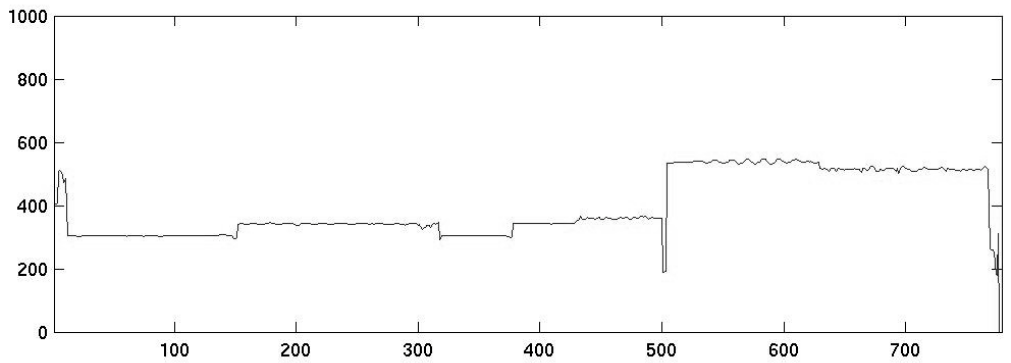
\includegraphics[scale=.25]{graph/pitch_onset}
                        \end{figure}
            \end{enumerate}
        \end{frame}
        \begin{frame}{onset detection}{novelty function examples 2/3}
            \begin{enumerate}   
                \setcounter{enumi}{2}
                \item	\textbf{STFT-based}: compute block difference 
                    \begin{itemize}
                        \item	\textit{flux}
                        \only<1->
                        {
                            \begin{itemize}
                                \item $d_\mathrm{hai}(n) = \sum\limits_{k = 0}^{\mathcal{K}/2-1}{\log_2\left(\frac{|X(k,n)|}{|X(k,n-1)|}\right)}$
                                \item $d_\mathrm{lar}(n) = \sum\limits_{k = k(f_{\mathrm{min}})}^{k(f_{\mathrm{max}})}{\sqrt{|X(k,n)|}-\sqrt{|X(k,n-1)|}}$
                            \end{itemize}
                        }
                        \item<2->	\textit{cosine distance}
                        \only<2->
                        {
                           \begin{itemize}
                                \item $d_\mathrm{foo}(n)	= 1 - \frac{\sum\limits_{k = 0}^{\mathcal{K}/2-1}{|X(k,n)|\cdot |X(k,n-1)|}}{\sqrt{\left(\sum\limits_{k=0}^{\mathcal{K}/2-1}{|X(k,n)|^2}\right)\cdot \left(\sum\limits_{k=0}^{\mathcal{K}/2-1}{|X(k,n-1)|^2}\right)}}$
                            \end{itemize}
                        }
                        \item<3->	\textit{complex}
                        \only<3->
                        {
                            \begin{equation*}
                                d_\mathrm{dux}(n) = \sum\limits_{k = 0}^{\mathcal{K}/2-1}{|X(k,n)-X(k,n-1)|}
                            \end{equation*}
                        }
                    \end{itemize}
            \end{enumerate}
        \end{frame}
        \begin{frame}{onset detection}{novelty function examples 3/3}
            \begin{enumerate}   
                \setcounter{enumi}{2}
                \item	\textbf{STFT-based} cont'd 
                    \begin{itemize}
                        \item<1->	\textit{Goto}-distance\footfullcite{goto_music_1995}
                            \begin{itemize}
                                \item	higher power than closest preceding and following bins
                            \end{itemize}
                        \only<1>-
                        {							
                            \begin{figure}
                                \centering
                                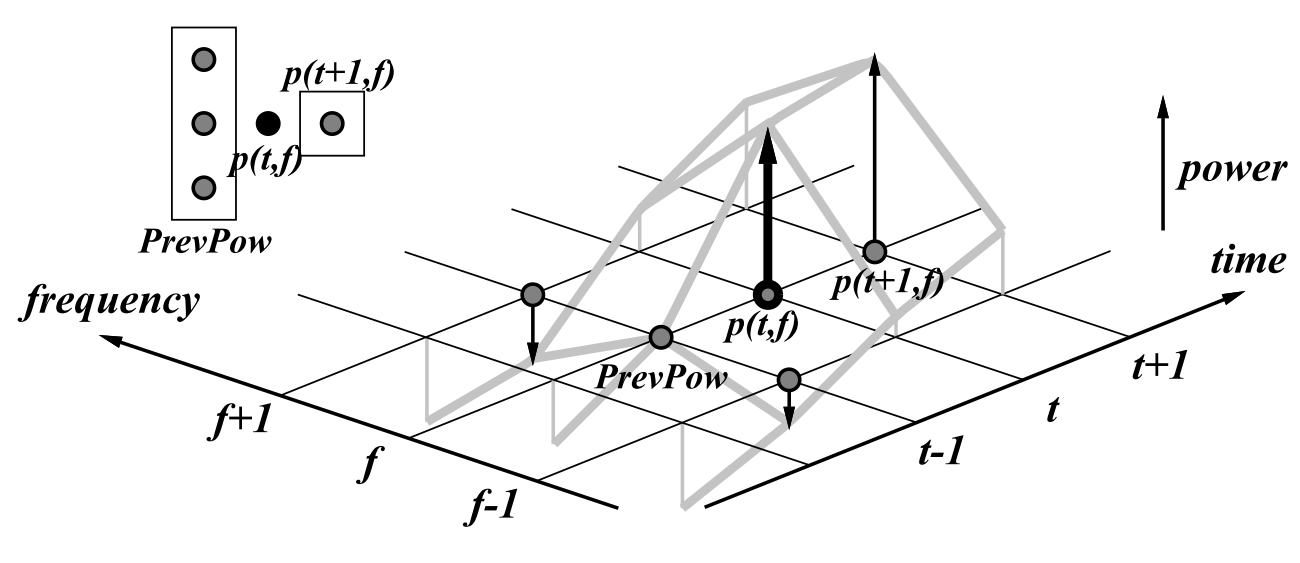
\includegraphics[scale=.25]{goto_onset}
                            \end{figure}
                        }
                    \end{itemize}
            \end{enumerate}
        \end{frame}
        \begin{frame}{onset detection}{novelty function: variants}
            \begin{itemize}
                \item	\textbf{number of frequency bands}
                    \begin{itemize}
                        \item	varies: 1, 3, 6, 21, 960, FFT length, ...
                        \item<2->	larger number of bands not necessarily better\\ $\rightarrow$ adjust number of bands adaptively?
                    \end{itemize}
                \bigskip
                \item<3->	\textbf{combination of bands}
                    \begin{itemize}
                        \item	(weight and) add novelty functions per band
                        \item<4->	onset detection per band and combine results
                    \end{itemize}
            \end{itemize}
        \end{frame}
    \section{peak picking}
        \begin{frame}{onset detection}{peak picking: introduction}
            \vspace{-4mm}
            \begin{itemize}
                \item	detect onsets in the smoothed novelty function
                    \vspace{-1mm}
                    \figwithmatlab{NoveltyFunction}
                \vspace{-3mm}
                \item<2->	typical \textbf{criteria}
                    \begin{itemize}
                        \item<2->	local maximum \& salient peak
                        \item<2->	higher than minimum likelihood
                        \item<2->	not too close to maxima with higher likelihood
                        \item<2->	other options: high attack slope, distance to prev. min, \ldots
                    \end{itemize}
            \end{itemize}
        \end{frame}
        \begin{frame}{onset detection}{peak picking: thresholding}
            \only<1>{
            \begin{itemize}
                \item options for thresholding
                    \begin{itemize}
                        \item \textbf{fixed} threshold
                        \begin{equation*}
                            G_{d,\mathrm{c}} = \lambda_1 
                        \end{equation*}
                        \item<1->	\textbf{smoothed} threshold
                        \begin{equation*}
                            G_{d,\mathrm{ma}} = \lambda_2 + \sum\limits_{j=0}^{\mathcal{O}-1}{b(j)\cdot d(i-j)}
                        \end{equation*}
                        \item<1->	\textbf{median} threshold
                        \begin{equation*}
                            G_{d,\mathrm{me}} = \lambda_2 + \hat{Q}_d(0.5) 
                        \end{equation*}
                    \end{itemize}
            \end{itemize}
            }
            \only<2>{
            \figwithmatlab{PeakPicking}
            }
        \end{frame}
        %\begin{frame}{onset detection}{evaluation}
            %\question{how do you properly evaluate an onset detection system}
            %\begin{itemize}
                %\item   methodology
                %\smallskip
                %\item   ground truth
                    %\begin{itemize}
                        %\item   how to get/generate
                        %\item   necessary annotations
                    %\end{itemize}
                %\smallskip
                %\item   metrics
                    %\begin{itemize}
                        %\item   how to measure the accuracy of your system
                    %\end{itemize}
            %\end{itemize}
        %\end{frame}

    
    \section{summary}
        \begin{frame}{summary}{lecture content}
            \begin{itemize}
                \item   \textbf{novelty function}
                    \begin{itemize}
                        \item   measure of unexpectedness - likelihood of an event
                            \begin{itemize}
                                \item   often a measure similar to flux
                            \end{itemize}
                    \end{itemize}
                \bigskip
                \item   \textbf{peak picking}
                    \begin{itemize}
                        \item   detecting peaks (onsets) in the novelty function
                        \item   usually done by smoothing and adaptive thresholding
                    \end{itemize}
            \end{itemize}
            \inserticon{summary}
        \end{frame}
\end{document}
